\section{OpenAI}
OpenAI adalah perusahaan riset dan pengembangan Artificial Intelligence (AI) yang berfokus pada pengembangan sistem AI yang aman dan bermanfaat bagi umat manusia. Salah satu produk utamanya adalah model bahasa generatif seperti GPT (\textit{Generative Pre-trained Transformer}), yang telah digunakan secara luas dalam berbagai aplikasi, mulai dari chatbot, penulisan otomatis, hingga sistem tanya-jawab berbasis dokumen. OpenAI juga menyediakan antarmuka pemrograman aplikasi (API) yang memungkinkan pengembang untuk mengintegrasikan model AI ini ke dalam aplikasi mereka \citep{openai2025api}.

\subsection{Retrieval-Augmented Generation}
\textit{Retrieval-Augmented Generation} (RAG) adalah sebuah kerangka kerja yang mengatasi keterbatasan model AI generatif tradisional dengan memungkinkan mereka untuk memberikan respons yang lebih akurat dan relevan secara kontekstual. Model generatif tradisional hanya menghasilkan output berdasarkan data pelatihan, yang dapat menyebabkan ketidakakuratan atau halusinasi saat menjawab pertanyaan di luar cakupan data tersebut. RAG mengatasi masalah ini dengan menggabungkan pendekatan berbasis \textit{retrieval} dengan model generatif \citep{rothman2024rag}.
\singlespacing{}
Framework RAG beroperasi dalam dua fase utama: \textit{retrieval} (pengambilan) dan \textit{generation} (generasi).

\begin{itemize}
    \item \textbf{Fase Retrieval:} Dalam fase ini, sistem mencari sumber eksternal secara real-time untuk informasi yang relevan terhadap kueri. Data yang diperoleh akan memperkaya input pengguna dan menjadi dasar untuk proses generasi jawaban. RAG dapat digunakan untuk berbagai jenis data, seperti teks, gambar, maupun audio.
    \item \textbf{Fase Generation:} Informasi hasil \textit{retrieval} kemudian dikombinasikan dengan input pengguna oleh model AI generatif untuk menghasilkan jawaban yang lebih akurat dan relevan.
\end{itemize}

\paragraph{Aspek dan Komponen Utama RAG}

\textbf{Konfigurasi RAG:}
\begin{itemize}
    \item \textit{Na\"ive RAG:} Menggunakan metode sederhana seperti pencarian kata kunci.
    \item \textit{Advanced RAG:} Menggabungkan teknik lanjutan seperti \textit{vector search} dan \textit{index-based retrieval}.
    \item \textit{Modular RAG:} Mengintegrasikan seluruh pendekatan sebelumnya dengan tambahan \textit{machine learning} dan algoritma kompleks.
\end{itemize}

\textbf{Ekosistem RAG:} 
\begin{itemize}
    \item \textbf{Data (D):} Mencakup pengumpulan, pemrosesan, penyimpanan, dan pengambilan data dari berbagai format.
    \item \textbf{Generator (G):} Bertanggung jawab atas \textit{prompt engineering} dan generasi jawaban.
    \item \textbf{Evaluator (E):} Mengevaluasi kualitas output menggunakan metrik seperti \textit{cosine similarity} dan umpan balik pengguna.
    \item \textbf{Trainer (T):} Terlibat dalam \textit{pre-training} dan \textit{fine-tuning} model generatif.
\end{itemize}

\textbf{RAG vs. Fine-tuning:} 
\begin{itemize}
    \item \textit{Parametric knowledge} mengacu pada pengetahuan yang tertanam dalam parameter model dan dapat disempurnakan melalui \textit{fine-tuning}.
    \item \textit{Non-parametric knowledge} merujuk pada data eksplisit yang disimpan dan dikueri secara langsung oleh sistem, menjadi fokus utama pendekatan RAG.
\end{itemize}

\textbf{Ketertelusuran (Traceability):} 
Keunggulan utama RAG adalah kemampuannya dalam melacak setiap output ke sumber dokumen asli, meningkatkan transparansi serta meminimalkan ketidakakuratan dan bias \citep{rothman2024rag}.

\subsection{LangChain}
LangChain adalah pustaka \textit{open-source} yang dirancang untuk memudahkan pengembangan aplikasi berbasis \textit{Large Language Models} (LLM), seperti chatbot dan agen AI, dengan menggabungkan teknik \textit{prompt engineering} serta integrasi ke sumber data eksternal dan alat bantu lainnya. LangChain menyediakan abstraksi modular dalam bentuk fungsi dan kelas yang fleksibel untuk membangun aplikasi LLM yang kompleks, baik dengan model dari penyedia komersial seperti OpenAI maupun model \textit{open-source} seperti Llama dan Gemma \citep{oshin2024learning}.

\begin{figure}[htbp]
  \centering
  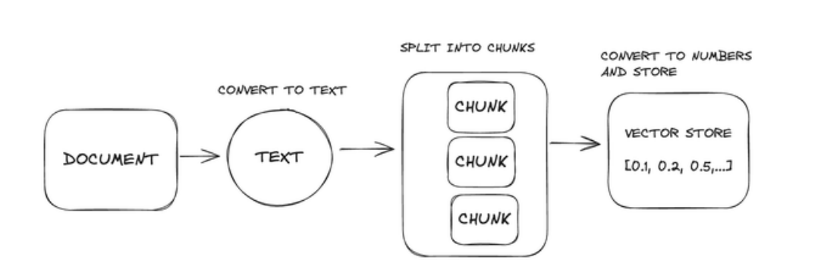
\includegraphics[width=0.85\linewidth]{images/bab-2/llm-process.png}
  \caption{Empat langkah utama untuk memproses awal dokumen untuk penggunaan LLM}\label{fig:langchain-pipeline}\citep{bagui2023database}
\end{figure}
\singlespacing{}
LangChain memungkinkan pengembang tidak hanya mengirim \textit{prompt} dan menerima respons dari model bahasa, tetapi juga melakukan teknik lanjutan seperti \textit{Retrieval-Augmented Generation (RAG)}, \textit{tool calling}, dan \textit{memory management}. Dengan fitur ini, sistem dapat melakukan \textit{chain-of-thought reasoning}, mengambil informasi dari dokumen eksternal, menggunakan kalkulator, dan mengingat konteks percakapan sebelumnya.
\singlespacing{}
Salah satu kekuatan utama LangChain adalah kemampuannya untuk membungkus seluruh proses pembangunan aplikasi LLM menjadi alur kerja yang terstandarisasi dan fleksibel. Selain itu, LangChain juga mendukung pemantauan dan pengujian sistem melalui platform seperti LangSmith dan LangServe.
\singlespacing{}
Dengan jutaan unduhan bulanan dan kontribusi aktif dari komunitas, LangChain menjadi pustaka terkemuka dalam pengembangan aplikasi AI generatif dan sangat relevan digunakan dalam pengembangan aplikasi pada penelitian ini \citep{oshin2024learning}.